\documentclass[twoside]{article}
\usepackage[utf8x]{inputenc}
\usepackage[T1]{fontenc}
\usepackage{txfonts}
\usepackage[paper=a5paper,lmargin=0.75cm,tmargin=0.5cm]{geometry}
\usepackage{setspace}
\usepackage{graphics}
\usepackage{color}
\usepackage{paralist}
\pagestyle{empty}
\setlength{\parindent}{0pt}
\setlength{\parskip}{0em}
\title{Airbus numbers}
\author{Jon Hurst}
\setcounter{secnumdepth}{0}

\renewcommand{\ref}[1]{{\color{blue}\scriptsize [#1]}}

\newcommand{\mysec}[2]{
  \vfil\vbox{
    \subsection{#1}
    \begin{list}{}{\setlength\parsep{0pt}\setlength\itemsep{0pt}}
    #2
    \end{list}}}

\newcommand{\iitem}{\item\hspace{2em}}

\newcommand{\pitem}[1]{
\item\hfill\parbox{22em}{\begin{spacing}{0.9}\vspace{0.25em} #1 \vspace{0.8em}\end{spacing}}}

\begin{document}

\vfil\vbox{
\subsection{Crosswind Limits}
\subsubsection{Runway Width $\geq$45m \ref{EOMB 2.1, LIM.22.20}}
\begin{center}
\begin{tabular}{|l|c|}\hline
  \parbox{0.5\textwidth}{
  \begin{center}Condition
  \end{center}}
  & Max Crosswind (inc. gust)\\\hline
  \parbox{0.5\textwidth}{
    \vspace{1mm}
    \begin{compactitem}
    \item Dry
    \item Damp
    \item Wet (≤3mm water)
    \end{compactitem}
    \vspace{1mm}} & 38kt\\\hline
  \parbox{0.5\textwidth}{
    \vspace{1mm}
    \begin{compactitem}
     \item Frost
     \item Slush ($\leq$3mm)
     \item Wet Snow ($\leq$3mm)
     \item Dry Snow ($\leq$3mm)
     \item Compacted Snow (OAT$\leq$-15°C)
    \end{compactitem}
    \vspace{1mm}} & 29kt\\\hline
  \parbox{0.5\textwidth}{
    \vspace{1mm}
    \begin{compactitem}
     \item Wet Snow (>3mm, $\leq$30mm)
     \item Dry Snow (>3mm, $\leq$130mm)
     \item Compacted Snow (OAT>-15°C)
     \item Slippery when wet
    \end{compactitem}
    \vspace{1mm}} & 25kt\\\hline
  \parbox{0.5\textwidth}{
    \vspace{1mm}
    \begin{compactitem}
     \item Autoland
     \item Rollout: No sharklets, dry/damp/wet
     \item Water (>3mm, $\leq$12.7mm)
     \item Slush (>3mm, $\leq$12.7mm)
    \end{compactitem}
    \vspace{1mm}} & 20kt\\\hline
  \parbox{0.5\textwidth}{
    \vspace{1mm}
    \begin{compactitem}
     \item Rollout:  With sharklets, dry/damp/wet
     \item Ice (cold and dry)
    \end{compactitem}
    \vspace{1mm}} & 15kt\\\hline
  \parbox{0.5\textwidth}{
    \vspace{1mm}
    \begin{compactitem}
     \item Ice (wet)
     \item Water over compacted snow
     \item Wet or dry snow over ice
    \end{compactitem}
    \vspace{1mm}} & Not recommended\\\hline
\end{tabular}
\end{center}}

\vfil\vbox{
\subsubsection{Runway Width $<$45m, $\ge$30m \ref{PRO.SPO.60}}
\begin{center}
\begin{tabular}{|l|c|}\hline
  \parbox{0.5\textwidth}{
  \begin{center}Condition
  \end{center}}
  & Max Crosswind (inc. gust)\\\hline
  \parbox{0.5\textwidth}{
    \vspace{1mm}
    \begin{compactitem}
    \item Dry
    \end{compactitem}
    \vspace{1mm}} & 38kt\\\hline
  \parbox{0.5\textwidth}{
    \vspace{1mm}
    \begin{compactitem}
    \item Wet (≤3mm water)
    \end{compactitem}
    \vspace{1mm}} & 33kt\\\hline
  \parbox{0.5\textwidth}{
    \vspace{1mm}
    \begin{compactitem}
    \item Contaminated
    \end{compactitem}
    \vspace{1mm}} & 10kt\\\hline
  \parbox{0.5\textwidth}{
    \vspace{1mm}
    \begin{compactitem}
    \item Icy
    \end{compactitem}
    \vspace{1mm}} & Not demonstrated\\\hline
  \parbox{0.5\textwidth}{
    \vspace{1mm}
    \begin{compactitem}
    \item Rudder or Rudder Pedal Jam
    \item Yaw damper system inop
    \item Rudder travel limiter fault
    \item Nosewheel steering inop
    \item One or more brakes inop
    \item Autoland
    \end{compactitem}
    \vspace{1mm}} & Not recommended\\\hline

\end{tabular}
\end{center}}


\mysec{Other wind limits}{
\item Max tailwind \ref{LIM.12}\dotfill 10kt
\item Max autoland headwind \ref{LIM.22.20}\dotfill 30kt
\item Passenger door operation \ref{LIM.12}\dotfill 65kt
\item Cargo door operation \ref{LIM.12}\dotfill 40kt (50kt w/caveats)
\item Cargo door closed before \ref{LIM.12}\dotfill 65kt
}

\vfil\vbox{
\subsection{Wake Turbulence}
\subsubsection{Final Approach \ref{EOMA 8.3.9}}
\begin{center}
  \begin{tabular}{|c|c|}\hline
    Type & Separation\\\hline
    A380 & 7nm\\
    Heavy & 5nm\\
    Upper Medium (e.g. 757,707) & 4nm (UK only)\\\hline
  \end{tabular}
\end{center}

\textbf{Note}: Boeing 757 and Boeing 737-800/900 are classified as heavy for the purposes of final
approach in some countries.

\subsubsection{Departure \ref{EOMA 8.3.9}}
\begin{center}
  \begin{tabular}{|c|c|}\hline
    Type & Separation\\\hline
    A380 & 3 mins\\
    Heavy & 2 mins\\\hline
  \end{tabular}
\end{center}

\textbf{Note}: Add \textbf{1 minute} if departure is not from the same position
}

\mysec{First Officer limits}{
\item 3* FO \ref{EOMB 2.1}\dotfill No planned tailwind
\item Max crosswind \ref{EOMB 2.1}\dotfill 20kt
\item Takeoff minimum \ref{EOMB 2.1}\dotfill 400m RVR
\item ILS/VOR/ADF/SRA minima \ref{EOMB 2.1}\dotfill As published
\item Circling minima \ref{EOMB 2.1}\dotfill 5000m
\item Min runway width, no specific training \ref{EOMB 2.1}\dotfill 45m
\item 3* FO \ref{EOMB 2.1}\dotfill no flap 3 landing
\item No contamination, windshear or autoland \ref{EOMB 2.1}
}

\mysec{General speeds}{
\item V$_{MO}$ \ref{LIM.13}\dotfill 350kt
\item M$_{MO}$ \ref{LIM.13}\dotfill 0.82M
\item Max Tire speed \ref{LIM.13}\dotfill 195kt
\item Max speed for wipers \ref{LIM.13}\dotfill 230kt
\item Max speed cockpit window open \ref{LIM.13}\dotfill 200kt
\item V$_{MCA}$ \ref{LIM.13}\dotfill 108kt$-\sim$1kt/1000ft
\item V$_{MCG}$ \ref{LIM.13}\dotfill 104.5kt@0ft,102.5kt@2000ft
\item Turbulence speeds \ref{PRO.SUP.91.10}
  \iitem $<$FL200\dotfill 250kt
  \iitem $\ge$FL200\dotfill 275kt
  \iitem $\ge$FL320\dotfill M0.76
}

\vfil\vbox{
\subsection{Weights \ref{LIM.11}}
\begin{center}
\begin{tabular}{|l|c|c|}\hline
  Weight & A319 & A320 \\ \hline
  Max Takeoff & 68000kg & 77000kg \\
  Max Taxi & 68400kg & 77400kg \\
  Max Landing & 61000kg & 66000kg \\
  Max Zero Fuel & 57000kg & 62500kg \\
  Minimum & 35400kg & 37230kg \\ \hline
\end{tabular}
\end{center}}


\vfil\vbox{
\subsection{Cargo bay weight limits \ref{PER.LOD.CGO}}
\begin{center}
\begin{tabular}{|l|c|c|l|c|}\cline{1-2}\cline{4-5}
\multicolumn{2}{|c|}{A319} & &
\multicolumn{2}{|c|}{A320}\\\cline{1-2}\cline{4-5}
Compartment 1 & 2268kg & & Compartment 1 & 3402kg\\
Section 41 & 1326kg & & Compartment 3 & 2426kg\\
Section 42 & 1695kg & & Compartment 4 & 2110kg\\
Compartment 5 & 1497kg & & Compartment 5 & 1497kg\\\cline{1-2}\cline{4-5}
\end{tabular}
\end{center}}


\vfil\vbox{
\subsection{Dimensions \ref{DSC.20.20}}
\begin{center}
\begin{tabular}{|l|c|c|c|}\hline
  & \parbox{.15\textwidth}{\centering A319}
  & \parbox{.15\textwidth}{\centering A320 (no sharklets)}
  & \parbox{.15\textwidth}{\centering A320 (sharklets)}\\\hline
  Wingspan  & \multicolumn{2}{c|}{34.1m} & 35.8m\\\cline{2-4}
  Length  & 33.84m & \multicolumn{2}{c|}{37.57m}\\\cline{3-4}
  Min pavement for 180° turn  & 20.64m & 22.9m & 22.8m\\\cline{2-4}
  Widest sweep  & \multicolumn{3}{c|}{Wing tip} \\\hline
\end{tabular}
\end{center}}


\mysec{Engine}{
\item TOGA time \ref{LIM.70}\dotfill 5 mins (10 mins single engine)
\item EGT \ref{LIM.70}
\iitem TOGA \dotfill 950°C
\iitem MCT \dotfill 915°C
\iitem Start \dotfill 725°C
\item Oil
\iitem Min quantity \ref{EOMB 2.3.4.3}\dotfill 9.5qt+0.5qt/hr
\iitem Max cont temp \ref{LIM.70}\dotfill 140°C
\iitem Max trans temp \ref{LIM.70}\dotfill 155°C
\iitem Min start temp \ref{LIM.70}\dotfill -40°C
\iitem Min takeoff temp \ref{LIM.70}\dotfill -10°C
\item Max N1 \ref{LIM.70}\dotfill 104\%
\item Max N2 \ref{LIM.70}\dotfill 105\%
\item Starter \ref{LIM.70}
\pitem{ 4 cycles of max 2 mins with 20 sec pause between each
  attempt,  then 15 min cooling period.}
\item Max reverse \ref{LIM.70}\dotfill >70kt
}


\mysec{APU}{
\item Ops with ``Low Oil Level'' ECAM \ref{LIM.49.10}\dotfill 10hrs
\item Starter duty  \ref{LIM.49.10}\dotfill 3 cycles then 60 mins
\item Maximum N \ref{LIM.49.10}\dotfill 107\%
\item Max EGT  \ref{LIM.49.10}\dotfill 675°C
\item Max start EGT, <35000ft  \ref{LIM.49.10}\dotfill <35000ft: 1090°C, >35000ft 1120°C
\item Max Altitudes \ref{LIM.49.20}
\iitem Two packs \dotfill 15000ft
\iitem One pack \dotfill 22500ft
\iitem Eng start \dotfill 20000ft
\iitem Battery start (emerg elec config) \dotfill 25000ft
\iitem Restart and operation \dotfill 39000ft
\iitem  Air bleed for wing anti-icing \dotfill Not permitted
\item Approximate fuel burn \ref{EOMB 5.1} \dotfill 2kg/min
}


\mysec{Flaps/slats}{
\item Conf 1 \ref{LIM.13}\dotfill 230kt
\item Conf 1+F \ref{LIM.13}\dotfill 215kt
\item Conf 2 \ref{LIM.13}\dotfill 200kt
\item Conf 3 \ref{LIM.13}\dotfill 185kt
\item Conf Full \ref{LIM.13}\dotfill 177kt
\item Max flaps/slats altitude \ref{LIM.27}\dotfill 20000ft
}


\mysec{Gear}{
\item Extend \ref{LIM.13}\dotfill 250kt
\item Retract \ref{LIM.13}\dotfill 220kt
\item Extended \ref{LIM.13}\dotfill 280kt/M.67
\item Max gear altitutde \ref{LIM.13}\dotfill 25000ft
\item Max taxi speed, single tyre deflated \ref{LIM.32}\dotfill 7kt
\item Max taxi speed, both tyres deflated \ref{LIM.32}\dotfill 3kt
\item Max steering angle, both tyres deflated \ref{LIM.32}\dotfill 30°
\item Max brake temp for takeoff \ref{LIM.32}\dotfill 300°
}


\mysec{Hydraulics}{
\item Normal pressure \ref{LIM.29}\dotfill 3000$\pm$200psi
}


\mysec{Electrical}{
\item Max generator continuous load \ref{LIM.24}\dotfill 100\%(90 KVA)
\item Max TR continuous load \ref{LIM.24}\dotfill 200A
}


\mysec{Pressurisation}{
\item Max pos diff \ref{LIM.21.20}\dotfill 8.6psi
\item Max neg diff \ref{LIM.21.20}\dotfill -1psi
\item Safety valve \ref{LIM.21.20}\dotfill 8.6psi
\item Max norm cabin alt \ref{LIM.21.20}\dotfill 8000ft
\item Cab alt warning \ref{LIM.21.20}\dotfill 9550ft$\pm$350ft
\item Ram air max diff \ref{LIM.21.10}\dotfill 1psi
}

\mysec{Air conditioning / Ventilation}{
\item Max LP ground unit airflow \ref{LIM.21.10}\dotfill 1.2kg/s
\item\hfill (do not simultaneously use packs)
\item Do not use HP ground unit when APU is supplying bleed air. \ref{LIM.21.10}
\item Max OAT for norm avionics ventilation \ref{LIM.21.30}\dotfill 49°C
\item \hfill(higher with time limits)
\item Max OAT with EXTRACT OVRD and Packs Off \ref{PRO.SUP.30}\dotfill
  39°C
\item \hfill(higher with time limits)
}


\mysec{Fuel}{
\item Approximate Capacity (varies by airframe) \ref{DSC.28.10.20}
\iitem Outer tanks \dotfill 2 x 700kg
\iitem Inner tanks \dotfill 2 x 5500kg
\iitem Center tank \dotfill 6500kg
\iitem Total \dotfill 18900kg
\item Allowable temperature (Jet A1) \ref{LIM.28}\dotfill ≥-43°C, ≤54°C
\item Max imbalance \ref{LIM.28}
\iitem Fuel in fuller inner tank $<$ 2250kg (outer tanks balanced) \dotfill No Limitation
\iitem Max inner tank imbalance (outer tanks balanced)\dotfill 1500kg
\iitem \hfill(more w/ caveats)
\iitem Max outer tank imbalance (sides balanced)\dotfill 1 full, 1 empty
\iitem Max takeoff imbalance with sharklets \dotfill inners: 500kg, outers:  370kg
\iitem \hfill(more w/ caveats)
\item Min qty for takeoff \ref{LIM.28}\dotfill 1500kg
}


\mysec{Oxygen}{
\item Min oxygen pressure (ref temp 40°) \ref{LIM.35}
\iitem 3 crew\dotfill 1024psi
\iitem 2 crew\dotfill 781psi
\item Endurance, emergency descent (reg normal) \ref{LIM.35}
\iitem Descent, 3 crew\dotfill 13 mins
\iitem Cruise at FL100, 2 crew \dotfill 107mins
\item Endurance, fire (reg 100\%) \ref{LIM.35}
\iitem 8000ft\dotfill 15mins
}


\mysec{Ice protection}{
\item Icing conditions \ref{PRO.SUP.30}\dotfill OAT(grd)|TAT(flt)$\le$10°C
\item\hfill (\& visible moisture or ground contamination)
\item Eng anti-ice not rqd \ref{PRO.SUP.30}\dotfill climb/cruise, SAT<-40°C
\item Accreted ice  \ref{PRO.SUP.30}
  \iitem Min speed, Conf Full \dotfill V$_{\mathrm{LS}}$ + 5kt
  \iitem Min Speed, < Conf Full \dotfill V$_{\mathrm{LS}}$ + 10kt
  \iitem Check landing performance \dotfill QRH FPE.IFL.VAP
\item Accreted ice, wing anti-ice inop \ref{PRO.SUP.30}
  \iitem Clean \dotfill V$_{\mathrm{LS}}$ + 15kt
  \iitem Conf 1, 2, 3, FULL \dotfill V$_{\mathrm{LS}}$ + 10kt
  \iitem Check landing performance \dotfill QRH FPE.IFL.30
\item Avoid extended flight in icing conditions with slats extended \ref{PRO.SUP.30}
}


\mysec{Navigation}{
\item Max IRS latitudes \ref{LIM.34}\dotfill 73°N,60°S
\item Altimeter tolerances \ref{PRO.SUP.34}
\iitem ADR vs Airfield elevation\dotfill $\pm$25ft
\iitem ADR vs ADR\dotfill $\pm$20ft
\iitem ISIS vs ADR\dotfill $\pm$100ft
}


\mysec{Autopilot}{
\item Engagement after TO \ref{3.1.22}\dotfill $>$100ft,$>$5 secs

\item Minimum disengagement
\iitem Cat II \ref{TR 87.1}\dotfill 80ft
\iitem Cat I \ref{3.1.22}\dotfill 160ft agl
\iitem NPA \ref{3.1.22}\dotfill MDA
\iitem Circling \ref{3.1.22}\dotfill MDA$-$100ft
\item Alert height \ref{3.1.22}\dotfill 100ft

\item Autoland limitations
\iitem Wind\dotfill see ``Other Wind limits''
\iitem Configurations \ref{3.1.22}\dotfill CONF 3, CONF Full
\iitem Rwy conditions for rollout\ref{3.1.22}\dotfill Dry,Wet
\iitem Glideslope\dotfill 2.5° to 3.15°
\iitem Max weight (emergency only)\dotfill 69000kg
}

\mysec{Airport}{
\item Max slope \ref{3.1.20}\dotfill $\pm$2\%
\item Max runway altitude \ref{3.1.20}\dotfill 9200ft
\item Nominal runway width \ref{3.1.20}\dotfill 45m
\item Min runway width \ref{2.4.60}\dotfill 30m (w/caveats)
\item Fire fighting category\ref{EOMA-8.1.2.1}\dotfill 6 (less w/caveats)
}


\mysec{Single Engine operations}{
\item Landing capability\ref{3.1.22}\dotfill Cat III single
\item Available NPA AP modes\ref{3.1.22}\dotfill LOC/VS;LOC/FPA;HDG/VS;HDG/FPA
\item\hfill(All modes permitted FD only)
\item Do not extend full flaps until established on final descent.
\item Use Conf 3 if a level off is required.
}


\mysec{Double engine failure}{
\item Range\dotfill 2½nm per 1000ft
\item Loss of height in hold\dotfill 8000ft
\item Loss of height in orbit\dotfill 4000ft
\item Target\dotfill OM at 2x normal height, flap 1, gear up
}

\mysec{Loading}{
\item Max LMC \ref{EOMB.7.4}
\iitem Total \dotfill $±$500kg
\iitem Passengers\dotfill +5/-10
\iitem Fuel\dotfill $±$500kg
\iitem CP4\dotfill $±$500kg
\iitem CP5 or CP1\dotfill $±$100kg
\item LMC Adjustments \ref{EOMB.7.4}
\iitem Negative \dotfill ZFW only
\iitem <250kg increase \dotfill ZFW; subtract 1 from FLEX
\item\hfill (FLEX must still be >ISA+30 and OAT)
\iitem >250kg \dotfill Use LPC
\item A320 Standard CG \ref{EOMB 4.9.4} \dotfill CG > 27\%MAC
\item A320 Forward CG \ref{EOMB 4.9.4} \dotfill CG < 27\%MAC
}

\mysec{Miscellaneous}{
\item German corner \dotfill KRH R270/12D
\item Runway lighting
\iitem Red and white \dotfill 900m
\iitem Red \dotfill 300m
\item Alternate ranges \ref{EOMB-5.1.1}
\iitem Takeoff \dotfill 320nm
\iitem Enroute \dotfill 380nm
\item Approximate corrections for $\ge$-10°\ref{EOMA-8.1.1.3.1}
\iitem 1000ft \dotfill 80ft
\iitem 2000ft \dotfill 160ft
\item Power settings, Flap 1 S or Flap full $V_{app}$
\iitem Two engine \dotfill GW-5
\iitem Single engine \dotfill GW+10
\item Flex corrections\ref{EOMB-2.3.10}
\iitem Anti-ice on \dotfill subtract 5°C
\iitem QNH reduction \dotfill subtract 1°C/2hPa
\iitem Flex must remain >ISA+30 and >OAT
}
\vfill
\pagebreak

\mysec{Emergency calls to cabin \ref{B2.7.33}}{
\item Ground ops alert:
  \pitem{``Attention! Crew at Stations''}
\item Ground ops alert cancellation:
  \pitem{``Cabin crew, normal operations''}
\item Evacuation:
  \pitem{``Evacuate. Unfasten your seatbelts and get out''}
\item NITS on flight deck:
  \pitem{``Senior cabin crew member to the flight deck''}
\item NITS via interphone:
  \pitem{``Senior cabin crew member to the interphone'' or 3 double chimes}
\item Unplanned emergency landing:
  \pitem{``Attention, Crew! Brace, Brace!''}
\item Slow decompression:
  \pitem{``Cabin crew, return to stations. We are commencing a
  descent - return to your seats and fasten your belts''}
\item Rapid decompression:
  \pitem{``Ladies and gentlemen, this is the Captain speaking. We have
  lost cabin pressure and are descending to a lower altitude. Put your
  oxygen masks on and obey the instructions of the cabin crew.''}
\item Planned emergency landing:
  \iitem 2000ft\dotfill ``Cabin crew, take up landing positions''
  \iitem 500ft\dotfill ``Brace, Brace''
\item Severe turbulence:
  \pitem{``Cabin crew and passengers be seated immediately''}
}

\vfill
\pagebreak
\section{Fuel Saving}

\mysec{Flap 3 landing}{
\item Min LDA \dotfill LDA$_{full}$*1.15
\item Autobrake LO, do not override
}

\mysec{Single Engine Taxi}{
\item Prohibited:
\iitem Icing conditions
\iitem Slippery taxiways
\iitem LVO
\iitem Inexperienced crew (first LPC/OPC not completed)
\iitem APU inop
\iitem Hydraulic, electric, steering or braking defects
\item Max time since shutdown\dotfill 6 hours
\item Max weight\dotfill 64000kg
\item Max thrust\dotfill 40\%N1
\item Min warmup\dotfill 2 mins
}

\vfill
\pagebreak


\section{Procedures}

\mysec{Takeoff with tailwind or crosswind > 20kt}{
\item[$\bullet$] Set 50\%
\item[$\bullet$] When engines stable, rapidly set 70\%
\item[$\bullet$] Select takeoff thrust by 40kt
\item[$\bullet$] Stick full forward until 80kt, neutral by 100kt
}

\mysec{General}{
\item UK Procedure speed limit\ref{AIP ICAO diffs}\dotfill 185kt
}

\mysec{ILS}{
\item Absolute minimas
\iitem Cat I \dotfill 200ft/550m
\iitem Cat II \dotfill 100ft/300m
\iitem Cat IIIA \dotfill 50ft/200m
\iitem Cat IIIB \dotfill 0ft/75m
}


\mysec{RNAV approach}{
\item[$\bullet$] Permitted RNAV approaches may be titled GPS, RNAV (GNSS), RNAV (GPS or DME/
DME)
\item[$\bullet$] Two navigation systems required - check RAIM
  availability \& GPS PRIMARY in both \mbox{MCDUs} before commencing
  approach
\item[$\bullet$] Non GPS PRIMARY approach must be available at destination alternate
\item[$\bullet$] Minimum OAT may apply (check approach plate). If no temperature is specified,
vertical guidance must not be used if temp $<=$ 0°C.
\item[$\bullet$] PI-CF leg (PROC-T on MCDU) not allowed
\item[$\bullet$] Do not revise final approach segment
\item[$\bullet$] Must be established laterally and vertically before
  descent position
\item[$\bullet$] \ref{OEB31}Do not use managed vertical guidance for
  an approach labelled ``RNV'' on the MCDU unless the MAP is located
  at the runway threshold (approaches labelled ``GPS'' are always OK)
\item[$\bullet$] If GPS PRIMARY LOST on one FMGC use autopilot associated with good FMGC
\item[$\bullet$] Go around for:
\iitem FM/GPS POS DISAGREE
\iitem GPS PRIMARY LOST on both FMGCs
\iitem GPS PRIMARY LOST on ND
\iitem $>$¾ index fly up or down
\iitem HIGH ACCURACY LOST
}

\mysec{Non-precision - Fully managed}{
\item[$\bullet$] GPS PRIMARY required
\item[$\bullet$] Min Temp 0°C
\item[$\bullet$] PI-CF leg (PROC-T on MCDU) not allowed
\item[$\bullet$] Do not revise final approach segment
\item[$\bullet$] Must be established laterally before descent
\item[$\bullet$] Arm Approach. Check FINAL blue, APP NAV
\item[$\bullet$] At D-0.2nm, check FINAL APP and monitor descent
}

\mysec{Non-precision - Managed lateral}{
\item[$\bullet$] GPS PRIMARY required
\item[$\bullet$] PI-CF leg (PROC-T on MCDU) not allowed
\item[$\bullet$] AT FAF, insert V$_{APP}$ if DP $<$10nm from runway,
  otherwise S speed
\item[$\bullet$] NAV/FPA when on final track
\item[$\bullet$] Conf 3,gear down by D-1nm
\item[$\bullet$] At D-0.2nm, select Conf full set and pull FPA
}

\mysec{Non-precision - Selected vertical and lateral}{
\item[$\bullet$] AT FAF, insert V$_{APP}$ if DP $<$10nm from runway,
  otherwise S speed
\item[$\bullet$] TRK/FPA when on final track
\item[$\bullet$] Conf 3,gear down by D-1nm
\item[$\bullet$] At D-0.2nm, select Conf FULL, set and pull FPA
}

\mysec{Circling}{
\item[$\bullet$] Landing runway in secondary flight plan
\item[$\bullet$] Initial approach: Conf 3, gear down, F speed
\item[$\bullet$] Push V/S at least 100ft above circling minima
\item[$\bullet$] Turn 45°
\item[$\bullet$] 30 secs from wings level turn downwind
\item[$\bullet$] Activate secondary when downwind
\item[$\bullet$] Descent point 3 secs per 100ft past abeam threshold
\item[$\bullet$] Full flap when turning finals
}

\mysec{Procedure turn}{
\item[$\bullet$] 75 seconds from start of 45° turn \ref{Jepp AER-91}
}

\mysec{Holding}{
\item Entries
\iitem Turn anti-holdwise<110° to OT\dotfill Parallel
\iitem Turn holdwise<70° to OT\dotfill Teardrop
\item Standard\dotfill Right turns, parallel to airway
\iitem $\le$14000\dotfill 1 minute
\iitem >14000\dotfill 1½ minutes
\item Max holding speeds (Normal(Turbulent))
\iitem <14000\dotfill 230kt(280kt)
\iitem 14000 to 20000\dotfill 240kt(280kt/0.8M)
\iitem 20000 to 34000\dotfill 265kt(280kt/0.8M)
\iitem >34000\dotfill 0.83M
}

\vfill

\mysec{LVO takeoff \ref{EOMB 2.4.4}}{
\item Abs minima\dotfill 125/125/125, 6 lights
\item Extra calls\dotfill ``Entering runway'', ``Rolling'', ``Airborne''
}

\mysec{LVO landing}{
\item[$\bullet$] Check NOTAMS for airport facility downgrades (see EOMA-8.1.3.10)
\item[$\bullet$] Check minimas, approach ban and LVPs in force
\item[$\bullet$] Check crew qualification and aircraft capability
\item[$\bullet$] Check autoland wind and runway condition limits
\item[$\bullet$] Review failure strategies
\item[$\bullet$] Extra calls:
\iitem 350ft, FMA:LAND \dotfill PF:``Land'', PNF:``Checked''
\iitem 100ft (only with no DH) \dotfill PNF: ``100'', PF: ``Continue''
\iitem 40ft, FMA:FLARE\dotfill PNF:``Flare''
\iitem 10ft \dotfill Auto callout: ``Retard''
\iitem FMA:ROLLOUT\dotfill PNF:``Rollout''
\iitem As appropriate\dotfill ``On ground'', ``Runway vacated''
\item[$\bullet$] If FLARE not annunciated by 30ft, go around
\item[$\bullet$] Select reverse at touchdown
\item[$\bullet$] Disconnect autopilot at taxi speed
}

\pagebreak

\vspace*{\fill}{}\resizebox{\textwidth}{!}{\rotatebox{90}{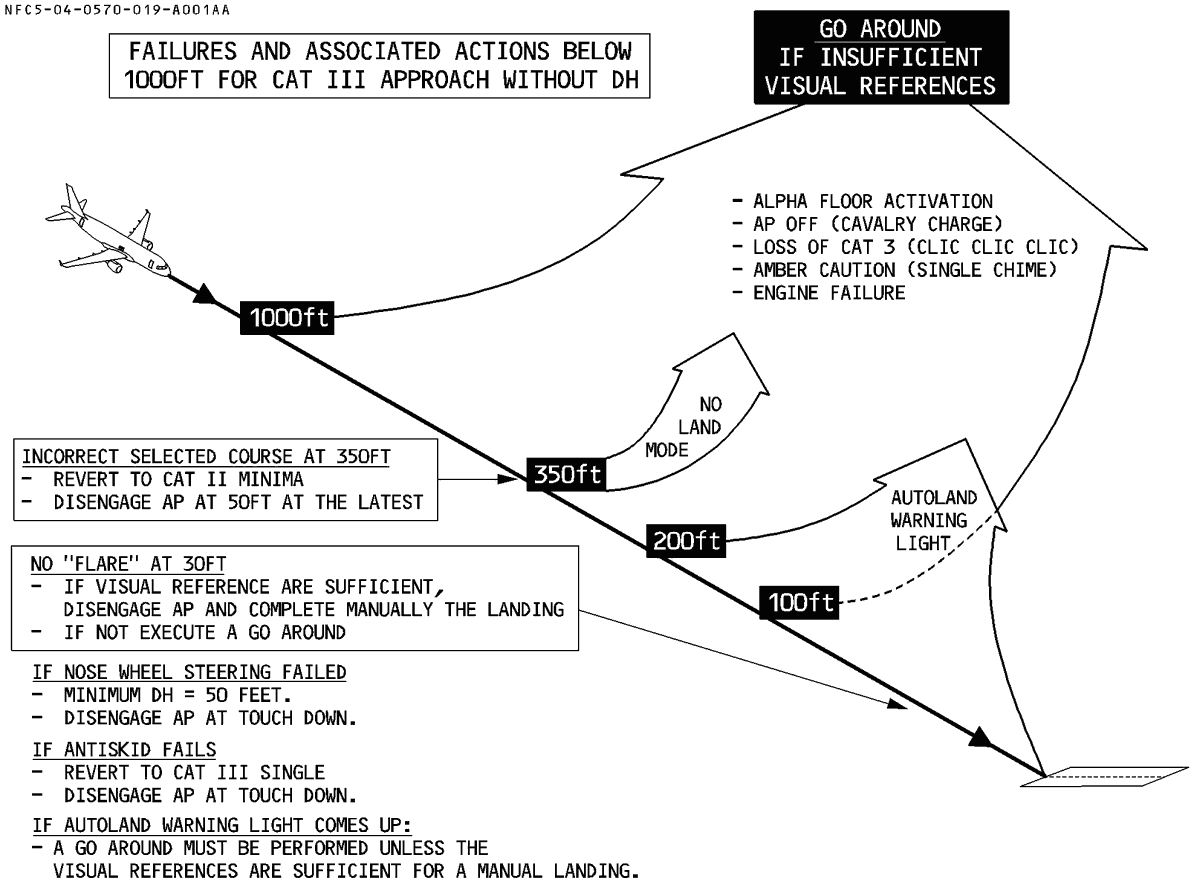
\includegraphics{images/catIII-failures.png}}}\vspace*{\fill}

\end{document}
